%%%%%%%%%%%%%%%%%%%%%%%%%%%%%%%%%%%%%%%%%%%%%%%%%%%%%%%%%%%%%%%
%
% Welcome to writeLaTeX --- just edit your LaTeX on the left,
% and we'll compile it for you on the right. If you give 
% someone the link to this page, they can edit at the same
% time. See the help menu above for more info. Enjoy!
%
% Note: you can export the pdf to see the result at full
% resolution.
%
%%%%%%%%%%%%%%%%%%%%%%%%%%%%%%%%%%%%%%%%%%%%%%%%%%%%%%%%%%%%%%%
% A simple fault tree
% Author: Zhang Long, Mail: zhangloong[at]gmail.com
%\def\pgfsysdriver{pgfsys-dvipdfm.def}
\documentclass{minimal}
\usepackage{tikz}
\usepackage{verbatim}
\usetikzlibrary{trees,positioning,arrows}
\begin{document}
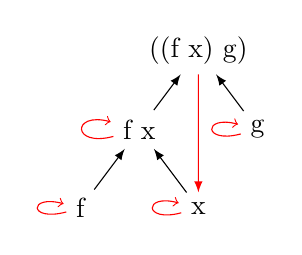
\begin{tikzpicture}[
	edge from parent path={(\tikzchildnode\tikzchildanchor) edge [-latex] (\tikzparentnode\tikzparentanchor)},
	level distance=1cm
]
%% Draw events and edges
\node (1) {((f x) g)}
	child {node (2) {f x}
    	child {node (5) {f}}
     	child {node (6) {x}}
    }
   	child {node (3) {g}}
    ;

\path[update/.style={red, -latex},
 	  updatelocal/.style={red, -latex, loop left}] 
 	(1) edge [update] (6)
    (3) edge [updatelocal] (3)
    (2) edge [updatelocal] (2)
    (5) edge [updatelocal] (5)
    (6) edge [updatelocal] (6)
    ;
        
\end{tikzpicture}
\end{document}
